
\chapter{Array}

\tikzstyle{array}=[rectangle,draw=blue!50,fill=blue!20,thick, inner sep=0pt,minimum size=1cm]
\tikzstyle{special}=[rectangle,draw=blue!50,fill=red!20,thick, inner sep=0pt,minimum size=1cm]
\tikzstyle{search}=[rectangle,draw=blue!50,fill=green!20,thick, inner sep=0pt,minimum size=1cm]
\tikzstyle{pre}=[<-,shorten <=1pt,>=stealth,semithick]
\tikzstyle{post}=[->,shorten >=1pt,>=stealth,semithick]
\section{What is an array?}

Arrays are collections of data that are stored in adjacent memory locations, so data elements are all available at random as each element can be identified with an array index.


For example in Figure \ref{fig:array-index}:
\begin{figure}[!htp]
  \centering
  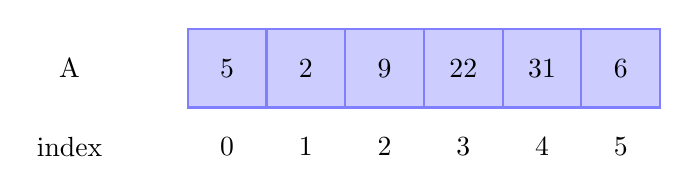
\begin{tikzpicture}
    \foreach \x\y in {0/5,1/2,2/9,3/22,4/31,5/6}
    {
      \node [array] () at (\x ,0) {\y};
      \node at (\x,-1) {\x};
    }
    \node at (-2,0) {A};
    \node at (-2,-1) {index};
  \end{tikzpicture}
  
  \caption{Array}
  \label{fig:array-index}
\end{figure}


In the example above, there are 6 elements in the array A, i.e. the
length of the array is 6. We can use $A[0]$ to indicate the first
element in the array A, so$A[0] = 5$. Similarly, $A[1] = 2$.




\section{Capacity and length}


The capacity is the maximum amount of data the array can hold, specified when you create the array.
The length is the amount of data that the current array holds.



\section{Operations}


An array is a data structure, which means it stores data in a specific format and supports specific operations on the data.

Operations on arrays:
\begin{itemize}
\item insert
\item delete
\item search
\end{itemize}



\section{Insert}

The insert into an array is like the Figure \ref{fig:array-insert}


\tikzstyle{array}=[rectangle,draw=blue!50,fill=blue!20,thick, inner sep=0pt,minimum size=1cm]
\begin{figure}[!htp]
  \centering
  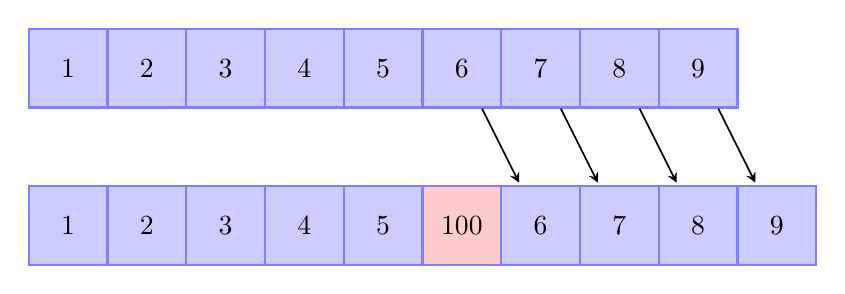
\begin{tikzpicture}
    \foreach \x in {1,...,9}{
      \node [array] (A\x) at (\x,0) {\x};
    }
    \foreach \x in {1,...,5}{
      \node [array] at (\x,-2) {\x};
    }
    \foreach \x in {6,...,9}{
      \node [array] (B\x) at (\x+1,-2) {\x}
      edge[pre] (A\x);
    }
    \node [special] at (6,-2) {100};
    
  \end{tikzpicture}

  \caption{Insert into an array}
  \label{fig:array-insert}
\end{figure}

Suppose the length of the array \(A\) is \(n\) and the start index is \(0\).
You can insert an element \(x\) at index \(0, 1, \ldots, n\).
\(x\) will be inserted into array \(A\) randomly so the probability to insert at \(i (0 \le i \le n)\) is the same.
Suppose the insert operation and movement operation take constant time \(1\).
The time complexity \(T\) will be:
\begin{align*}
  \label{eq:1}
  T &= \frac{1}{n+1}(n+1 + n + \ldots + 1)\\
    &= \frac{1}{n+1} \cdot \frac{(n+1)(n+2)}{2}\\
    &= \frac{n+2}{2}\\
    &= \frac{1}{2} n + 1
\end{align*}


The average time complexity of array insertion is $O(n)$, and the space complexity is $O(1)$.


\section{Delete}

To delete an element from an array is shown in Figure \ref{fig:array-delete}
\begin{figure}[!htp]
  \centering
  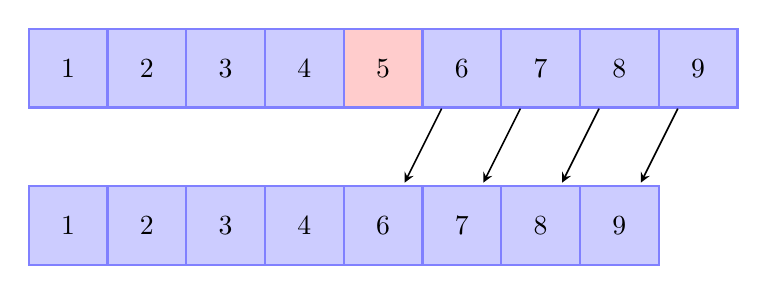
\begin{tikzpicture}
    \foreach \x in {1,...,9}{
      \node [array] (A\x) at (\x,0) {\x};
    }
    \node [special] at (5,0) {5};
    \foreach \x in {1,...,6}{
      \node [array] at (\x,-2) {\x};
    }
    \foreach \x in {6,...,9}{
      \node [array] (B\x) at (\x-1,-2) {\x}
      edge[pre] (A\x);
    }

    
  \end{tikzpicture}

  \caption{Delete from an array}
  \label{fig:array-delete}
\end{figure}

The average time complexity of array deletion is $O(n)$, and the space complexity is $O(1)$.


\section{Search}

To search an element in an array is shown in Figure \ref{fig:array-search}
\begin{figure}[!htp]
  \centering
  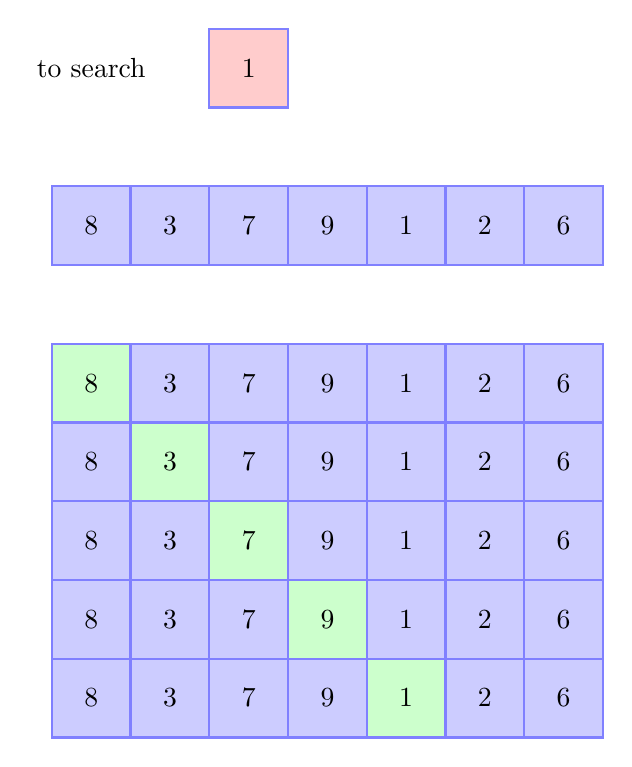
\begin{tikzpicture}
    \node [special] at (3,2) {1};
    \node at (1,2) {to search};
    \foreach \x\y in {1/8,2/3,3/7,4/9,5/1,6/2,7/6}{
      \node [array]  at (\x,0) {\y};
    }
    \foreach \z in {-2,-3,...,-6}{
      \foreach \x\y in {1/8,2/3,3/7,4/9,5/1,6/2,7/6}{
        \node [array] at (\x,\z) {\y};
      }
    }

    \foreach \x\y in {1/8,2/3,3/7,4/9,5/1}{
      \node [search] at (\x,-1-\x) {\y};
    }
    
  \end{tikzpicture}

  \caption{Search in an array}
  \label{fig:array-search}
\end{figure}


For an unordered array, you need to search the elements from the start of the array and one by one. So the time complexity of searching for an element in it is $O(n)$.

If the array is ordered, you can use other more efficient searching methods like binary search. 



\section{Strings}

A String is an array whose elements are characters.


\section{Examples}

Here are some codes about array on \href{https://github.com/mingmingli916/algorithms/tree/main/array}{Github}


\section{Conclusion}
\label{sec:conclusion}

\begin{itemize}
\item Changing the capacity is impossible.
\item Random access is $O(1)$.
\item Inserting and deleting is $O(n)$.
\end{itemize}


%%% Local Variables:
%%% mode: latex
%%% TeX-master: "algorithms"
%%% End:
